% !TeX root = RJwrapper.tex
\title{matRiks: An R package for the automatic generation of rule-based matrices}


\author{by Quietest Quokka and Bounciest Bilby}

\maketitle

\abstract{%
Few resources are available for the automatic generation of Raven-like matrices. Some of them are no longer working, while others are hardly customizable without strong programming skills. An R package fro the automatic generation of stimuli used for psychological assessment exists, but it is limited to one shape and to the manipulation of one rule (i.e., rotation). The \CRANpkg{matRiks} package has been developed with the aim of overcoming the above mentioned issues. This package can generate matrices considering different types of rules, starting from the most basic ones (e.g., changes in size, objects orientation) to the most complex ones, based on inferential and inductive reasoning. This unveils the possibility of generating new customizable stimuli and of systematically manipulating the difficulty of the matrices. Being developed within the R environment, the \CRANpkg{matRiks} package is completely open-source, allows for the reproducibility of the stimuli, and it can be easily used by people with basic knowledge of R language.
}

\hypertarget{introduction}{%
\section{Introduction}\label{introduction}}

Cattell (Cattell (1963)) defined fluid intelligence (\emph{g}) as the ability of solving novel reasoning problems that has little to do with concepts learned in schools or through acculturational processes. The adjective ``fluid'' explicitly refers to its ability to ``flow'' into a variety of tasks and cognitive activities (Horn, 1972).
Given this definition of fluid intelligence, it appears natural that the instruments for used for its evaluation tap on the respondent's ability to solve abstract problems that involve acculturation as little as possible, such as figural analogies, figure classifications, matrices, and number and letter series are often used (Horn, 1968).

The Raven's progressive matrices (RPM, JC ea Raven (1938)) are among the most famous tools for the assessment of \emph{g}. The RPM consists in a series of non-verbal multiple-choice stimuli where respondents are required to complete a series of drawings composed of different figures by identifying the relevant features that rule the relationships between the figures. These drawings are often referred to as matrices.
To pursue this aim, the respondents must choose the figure that complete the drawing among a list of other figures, the so-called distractors.
This task should measure the ability of the respondents to identify and take into account the features (also called ``rules'') that govern the relationship between the figures to compose the drawing.
The RPM and similar tasks (here denoted as Raven-like matrices or Raven-like tasks) are employed in different fields, from clinical evaluation of intelligence to the selection processes in organizational psychology (citation needed).
Since Raven's and Raven-like tasks involve the ability to solve new abstract problems, the stimuli composing these tasks should not be spread among the general population.
However, new stimuli can be generated according to the rules that govern the relationships between the figures composing the drawing. Indeed, different resources are available for developing Raven-like tasks, such as Sandia (cit), Corvus (cit), and the R package \CRANpkg{Imak} (cit).

The stimuli generated with Sandia have been analysed in an Item Response Theory framework to validate them as a test for measuring fluid intelligence.
The stimuli are available upon request to the authors, however no new stimuli can be generated because the code on which Sandia is based is no longer maintained.
Corvus represents another possible resource for generating Raven-like tasks. Corvus is written in Javascript but the Author provided a nice and easy-to-use graphical interface where the user can specify the figures and the rule(s) for the generation of the matrices. However, Corvus provides few degrees of freedom in terms of both the figures and the number of rules that can be manipulated through the graphical interface. If the user wants to add other figures, to modify the already existing figures, or to implement new rules, they have to modify the source code in Javascript, which might be a quite demanding task for people with little to null experience in programming.
Finally, the \texttt{ImaK} package is an \texttt{R} package that allows for generating visual analogies. The code for generating such stimuli (along with their response options) is quite straightforward and easy to use. However, the stimuli that can be generated with the \texttt{ImaK} package are mostly based on the rotation of the same figure to which some objects can be added or removed. As such, the only rule that is manipulated is the spatial rotation of the figures.

Given the limitations of the existing resources for generating Raven-like tasks, there might be the need of an open-source, easy-to-use, and constantly maintained resource for generating such stimuli through the systematic manipulation of rules applied to different figures.
The \texttt{matRiks} package (Brancaccio, Epifania, and de Chiusole (2023)) has been developed to pursue these aims.
Beyond generating the matrix by manipulating one or multiple rules at once on one or multiple figures, the \texttt{matRiks} package generates the response list associated to the matrix as well.
The systematic manipulation of both the rules and the figures for the matrix generation should grant the possibility of grading the granularity of the difficulty of the matrices by manipulating one element at the time.
In a similar vein, the package should allow for generating matrices that can be considered equivalent in terms of rules employed for their generation but differ in terms of figures composing the drawing. In what follows, the term stimulus is used to identify the matrix with its associated response list.

The manuscript is organized as follows.
The next section presents the rules that usually employed in the RPM along with the specific types of error responses (i.e., distractors) that compose the response list associated with a matrix. Then, the \texttt{matRiks} package is presented through an example of its application for the generation of different stimuli (i.e., the matrix with its associated response list).

\hypertarget{background}{%
\section{Background}\label{background}}

\hypertarget{rule-based-matrices}{%
\subsubsection{Rule based matrices}\label{rule-based-matrices}}

Literature highlights a plethora of rules that can be manipulated for the generation of the raven-like tasks (cit cit cit).
Beyond the fact that some of these rules have different names in different sources but refer to the same manipulation (e.g., the rule defined as ``and problem'' in Harris el a. 2020 is called ``intersection'' rule in Arendasy et al.~2005), they can be summarized into different macro-categories, namely visuospatial rules (i.e., the manipulation concerns the graphical and spatial features of the figures, Figure \ref{fig:visuoRule}), and logical rules (i.e., the manipulation concerns the logical relationships between the figures composing the matrix, , Figure \ref{fig:logiRule}). The rules can be applied (i.e., manipulated) to different figures or concatenation of figures to generate a matrix.

\begin{figure}

{\centering 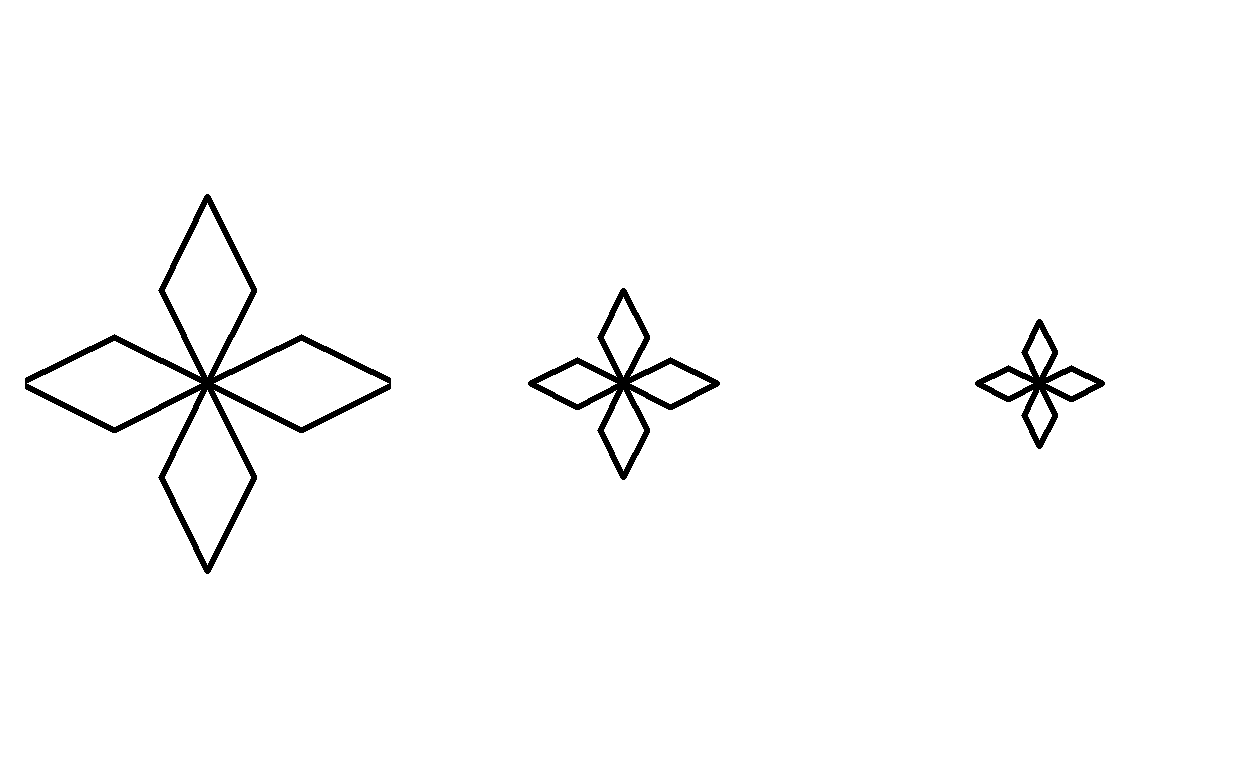
\includegraphics[width=0.7\linewidth]{matRiks-paper_files/figure-latex/visuoRule-1} 

}

\caption{Example of visuospatial rule: Changes in size}\label{fig:visuoRule}
\end{figure}

\begin{figure}

{\centering 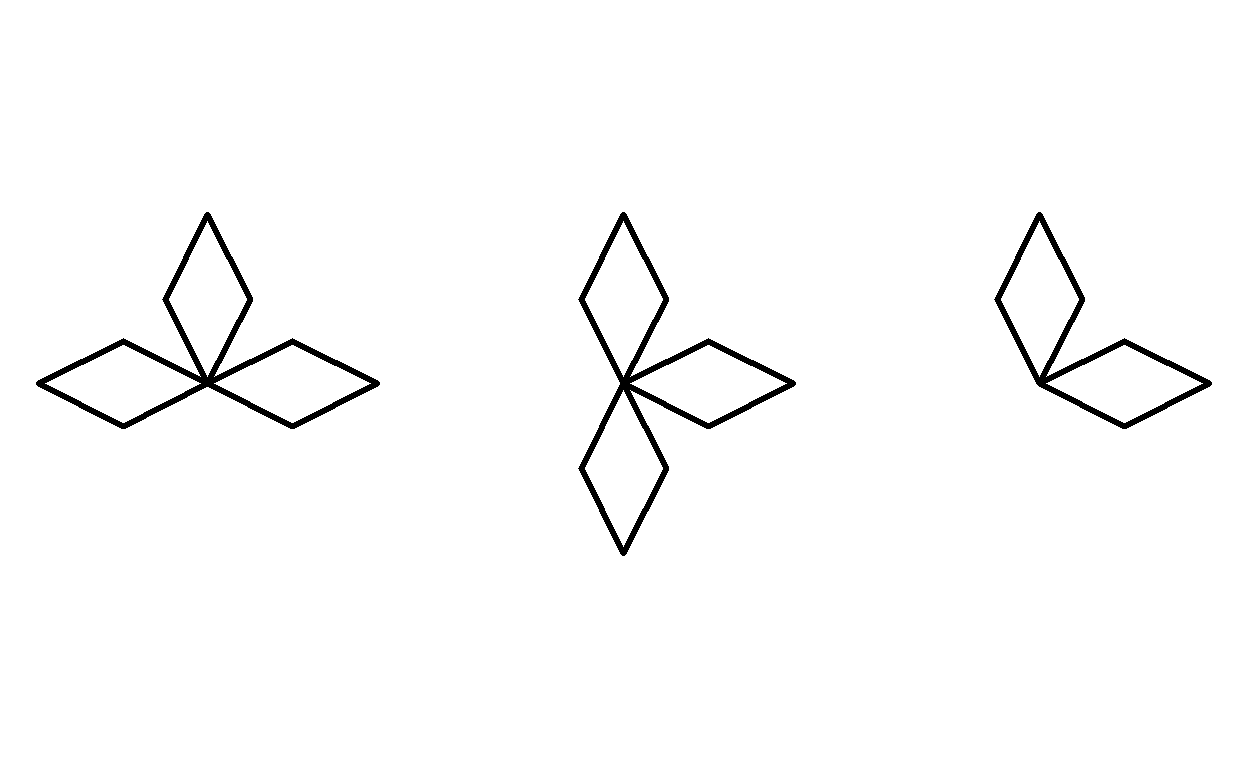
\includegraphics[width=0.7\linewidth]{matRiks-paper_files/figure-latex/logiRule-1} 

}

\caption{Example of logical rule: Insiemistic Interscetion AND}\label{fig:logiRule}
\end{figure}

In Figure \ref{fig:visuoRule}, the manipulation concerns a specif feature of the figure, that is its size, and it can be observed as the the figure decreases its size across the cells.
The rightmost cell contains the figure with the smallest size, the middle cell contains a figure with medium-small size while the leftmost object contains the figure with its original size.
In Figure \ref{fig:logiRule}, the manipulation concerns the relationships between the objects composing the figures, which are combined together according to a logical rule based on the insiemistic intersection of the objects. Specifically, the figure in the rightmost cell results from the intersection of the objects in the leftmost cell and in the middle cell.

Both visuospatial and logical rules can be manipulated according to different directional logic.
Specifically, the rules can be applied horizontally (i.e., the manipulation of the rule can be seen across columns but not across rows, H direction), vertically (i.e., the manipulation of the rule can be seen across rows but not across columns, V direction), or diagonally (i.e., the manipulation of the rule can be seen both across columns and across rows). Concerning the diagonal directional logic, it can follow either the main diagonal of the matrix (i.e., the manipulation of the rule can be seen from the top-left corner to the low-right corner, TL-LR direction) or the secondary diagonal of the matrix (i.e., the manipulation of the rule can be seen from the low-left corner to the top-right corner, LL-TR direction).

\hypertarget{the-response-options}{%
\subsubsection{The response options}\label{the-response-options}}

A large corpus of literature has investigated the role of the distractors in the response processes involved when solving the Raven matrices, focusing on the specific error response chosen by the respondent (Forthmann et al. (2020), Kunda et al. (2016), Storme et al. (2019)).
The underlying logic is that the incorrect response is not chosen at random by the respondent, but it can be the result of an educated guess, or it can be chosen because the respondent is misled for a definite reason.
In other words, the incorrect responses might reflect an incorrect solution strategy which results in the choice of a specific distractor type over another one (Kunda et al. 2016). The distractors can be classified according to the incorrect response strategy they represent.
Kunda et al. (2016) present a list of criteria for the identification of the distractors in the SPM based on the error types from the CPM and APM manuals (John Raven and Raven 2004). Specifically, the specific response that is chosen in place of the correct one (i.e.~error types) can be collected into four main four conceptual errors, namely Repetition (R), Difference (D), Wrong Principle (WP), and Incomplete Correlate (IC).
Repetition errors occur when the chosen response option is a cell adjacent to the blank space.
Difference errors occur when the chosen response option is completely different from any entry of the matrix.
Wrong principle errors occur when the chosen response option follows rules other than the ones used in the matrix. Incomplete Correlate errors occur when the chosen response option is in fact the correct response with a variation on a single feature. Each of the four main error types can be further described by their subcategories.\\
The definitions of each error type and of their specific subcategories are summarized in Table \ref{tab:tab-error-types}.

\hypertarget{customizing-tooltip-design-with}{%
\section{\texorpdfstring{Customizing tooltip design with \pkg{ToOoOlTiPs}}{Customizing tooltip design with }}\label{customizing-tooltip-design-with}}

\pkg{ToOoOlTiPs} is a packages for customizing tooltips in interactive graphics, it features these possibilities.

\hypertarget{a-gallery-of-tooltips-examples}{%
\section{A gallery of tooltips examples}\label{a-gallery-of-tooltips-examples}}

The \CRANpkg{palmerpenguins} data (Horst, Hill, and Gorman 2020) features three penguin species which has a lovely illustration by Alison Horst in Figure \ref{fig:penguins-alison}.

\begin{figure}

\includegraphics[width=1\linewidth,height=0.3\textheight]{figures/penguins} \caption{Artwork by \@allison\_horst}\label{fig:penguins-alison}
\end{figure}

Table \ref{tab:penguins-tab-static} prints at the first few rows of the \texttt{penguins} data:

\begin{table}

\caption{\label{tab:penguins-tab-static}A basic table}
\centering
\fontsize{7}{9}\selectfont
\begin{tabular}[t]{l|l|r|r|r|r|l|r}
\hline
species & island & bill\_length\_mm & bill\_depth\_mm & flipper\_length\_mm & body\_mass\_g & sex & year\\
\hline
Adelie & Torgersen & 39.1 & 18.7 & 181 & 3750 & male & 2007\\
\hline
Adelie & Torgersen & 39.5 & 17.4 & 186 & 3800 & female & 2007\\
\hline
Adelie & Torgersen & 40.3 & 18.0 & 195 & 3250 & female & 2007\\
\hline
Adelie & Torgersen & NA & NA & NA & NA & NA & 2007\\
\hline
Adelie & Torgersen & 36.7 & 19.3 & 193 & 3450 & female & 2007\\
\hline
Adelie & Torgersen & 39.3 & 20.6 & 190 & 3650 & male & 2007\\
\hline
\end{tabular}
\end{table}

Figure \ref{fig:penguins-ggplot} shows an plot of the penguins data, made using the \CRANpkg{ggplot2} package.

\begin{verbatim}
penguins %>% 
  ggplot(aes(x = bill_depth_mm, y = bill_length_mm, 
             color = species)) + 
  geom_point()
\end{verbatim}

\begin{figure}
\centering
\includegraphics{matRiks-paper_files/figure-latex/penguins-ggplot-1.pdf}
\caption{\label{fig:penguins-ggplot}A basic non-interactive plot made with the ggplot2 package on palmer penguin data. Three species of penguins are plotted with bill depth on the x-axis and bill length on the y-axis. Visit the online article to access the interactive version made with the plotly package.}
\end{figure}

\hypertarget{summary}{%
\section{Summary}\label{summary}}

We have displayed various tooltips that are available in the package \pkg{ToOoOlTiPs}.

\hypertarget{references}{%
\section*{References}\label{references}}
\addcontentsline{toc}{section}{References}

\hypertarget{refs}{}
\begin{CSLReferences}{1}{0}
\leavevmode\vadjust pre{\hypertarget{ref-matRiks}{}}%
Brancaccio, Andrea, Ottavia M. Epifania, and Debora de Chiusole. 2023. \emph{matRiks: Generates Raven-Like Matrices According to Rules}. \url{https://CRAN.R-project.org/package=matRiks}.

\leavevmode\vadjust pre{\hypertarget{ref-cattell1963}{}}%
Cattell, Raymond B. 1963. {``Theory of Fluid and Crystallized Intelligence: A Critical Experiment.''} \emph{Journal of Educational Psychology} 54 (1): 1. https://doi.org/\url{https://doi.org/10.1037/h0046743}.

\leavevmode\vadjust pre{\hypertarget{ref-fort}{}}%
Forthmann, Boris, Natalie Förster, Birgit Schütze, Karin Hebbecker, Janis Flessner, Martin T. Peters, and Elmar Souvignier. 2020. {``How {Much} g {Is} in the {Distractor}? {Re}-{Thinking} {Item}-{Analysis} of {Multiple}-{Choice} {Items}.''} \emph{Journal of Intelligence} 8 (1): 11. \url{https://doi.org/10.3390/jintelligence8010011}.

\leavevmode\vadjust pre{\hypertarget{ref-palmerpenguins}{}}%
Horst, Allison Marie, Alison Presmanes Hill, and Kristen B Gorman. 2020. \emph{{palmerpenguins}: Palmer Archipelago (Antarctica) Penguin Data}. \url{https://allisonhorst.github.io/palmerpenguins/}.

\leavevmode\vadjust pre{\hypertarget{ref-kunda}{}}%
Kunda, Maithilee, Isabelle Soulières, Agata Rozga, and Ashok K. Goel. 2016. {``Error Patterns on the {Raven}'s {Standard} {Progressive} {Matrices} {Test}.''} \emph{Intelligence} 59 (November): 181--98. \url{https://doi.org/10.1016/j.intell.2016.09.004}.

\leavevmode\vadjust pre{\hypertarget{ref-raven1938}{}}%
Raven, JC ea. 1938. {``Raven's Progressive Matrices.''} \emph{Western Psychological Services} 2: 5.

\leavevmode\vadjust pre{\hypertarget{ref-raven2004}{}}%
Raven, John, and H. Raven. 2004. {``Manual for {Raven}'s {Progressive} {Matrices} and {Vocabulary} {Scales}, {Section} 3: {The} {Standard} {Progressive} {Matrices}, {Including} the {Parallel} and {Plus} {Versions}. 2000 {Edition}, Updated 2004.''} In, Section 3.

\leavevmode\vadjust pre{\hypertarget{ref-storme}{}}%
Storme, Martin, Nils Myszkowski, Simon Baron, and David Bernard. 2019. {``Same {Test}, {Better} {Scores}: {Boosting} the {Reliability} of {Short} {Online} {Intelligence} {Recruitment} {Tests} with {Nested} {Logit} {Item} {Response} {Theory} {Models}.''} \emph{Journal of Intelligence} 7 (3): 17. \url{https://doi.org/10.3390/jintelligence7030017}.

\end{CSLReferences}

\bibliography{RJreferences.bib}

\address{%
Quietest Quokka\\
University of Little Mates\\%
Department of Letter Q\\ Somewhere, Australia\\
%
\url{https://www.britannica.com/animal/quokka}\\%
\textit{ORCiD: \href{https://orcid.org/0000-1721-1511-1101}{0000-1721-1511-1101}}\\%
\href{mailto:qquo@ulm.edu}{\nolinkurl{qquo@ulm.edu}}%
}

\address{%
Bounciest Bilby\\
University of Little MatesUniversity of Aussie Animals\\%
Department of Letter Q, Somewhere, Australia\\ Department of Marsupials, Somewhere, Australia\\
%
\url{https://www.britannica.com/animal/bilby}\\%
\textit{ORCiD: \href{https://orcid.org/0000-0002-0912-0225}{0000-0002-0912-0225}}\\%
\href{mailto:bbil@ulm.edu}{\nolinkurl{bbil@ulm.edu}}%
}
